\chapter{State of the art: Data collection and Techniques for Authorship Attribution}

\epigraph{\enquote*{\textit{State of the Art is the frenetic and relentless pursuit of doing what its best at that time!}}\\
Da Anunciaç\~ao Marco}

There are different types of authorship attribution studies in the literature such
as predicting the date of authorship of historical texts or text genre detection \cite{tausz2011predicting}, \cite{kessler1997automatic}.
Vast majority of previous works focuses on authorship identification by taking into
consideration the stylistic features of authors such as use of grammar, function words,
frequent word allocations \cite{argamon2005measuring}, \cite{fox2012statistical}, \cite{hirst2007bigrams}. Some of the well-known problems
in authorship attribution are disputed Federalist Papers classification and Shakespearean Authorship Dispute.
The Federalist Papers are a collection of 85 articles and essays written by Alexan-
der Hamilton, James Madison, and John Jay to persuade the citizens of New York
to ratify the U.S. Constitution. Authorship of twelve of these papers has been in
dispute. To address this problem, using linear support vector machines as classifier
and relative frequencies of words as features a study identified these papers to be
written by James Madison.\\
Another dispute in authorship attribution among scholars across the world is
whether William Shakespeare wrote the works attributed to him or not. It was argued
that Shakespeare was not even educated and more than 80 authors were suggested to
be the author of the writings that were under the name of Shakespeare. Christopher
Marlowe is considered the most likely candidate to write these works under the name
of Shakespeare when he was in jail. In order to analyze the stylistic fingerprint of
Shakespeare and Marlowe and non-Shakespearean authors, namely Chapman,Jonson, Middleton, a corpus has been put together. \cite{fox2012statistical}
The classification results for non-Shakespearean author candidates turned out to
be highly accurate (Johnson \%100, Chapman \%92.9 and Middleton \%88.9). The
results supported the hypothesis that writing styles of Marlowe and Shakespeare were
as distinguishable as other authors unless Marlowe did not show a linear change in
style over time. Meaning, Marlowe has found not to be the authors of Shakespearean
writings.
Another interesting study on the unknown texts is also
done based on word-level features, vocabulary richness and syntactic features by using
Liblinear SVM for classification purposes \cite{stanko2013whose}. Even though the classification accuracy
results are not as high as other related works features like \enquote*{number of unique words}
should be noted for use in any attribution problem.
Usefulness of function words in authorship attribution is introduced by Mosteller
and Wallace in their work on Federalist papers \cite{mosteller2007inference}. Argamon and Levitan has compared the characteristic features of frequent words, pairs and collocations using the
SMO algorithm, and implemented it for two class (American or British) author nationality classification problem. Their results conclude that function words are useful
as stylistic text attribution and frequent words are the best features among others.
The reason behind it is that a given same size frequent collocations has less different
words comparing to frequent words so it carries less discriminatory features \cite{argamon2005measuring}.
In summary, there has been substantial work done in authorship attribution and
mainly people in forensic linguistic or computer scientists aim to build \enquote*{stylistic fingerprint of author} by using several features of a given text such as function words,
stylometry. It is a classification problem and several classifiers are used such as Na\"ive
Bayes, SVM. Among them, SVM is observed to fit best for these kinds of problems.

\section{SVM}
Support Vector Machines (SVMs) recently gained popularity in the learning community\cite{vapnik1999overview}. In its simplest
linear form, an SVM is a hyperplane that separates
a set of positive examples from a set of negative examples with maximum interclass distance, the margin.
\autoref{fig:svm_margin} shows such a hyperplane with the associated
margin.
The formula for the output of a linear SVM is show in \autoref{svmformula}, where $w$ is the normal vector to the hyperplane, and $x$ is the input vector. The margin is defined by the distance of the hyperplane to the nearest of the positive
and negative examples.
\begin{equation}\label{svmformula}
	u = w * x + b
\end{equation}
Maximizing the margin can be
expressed as an optimization problem, as shown in  \autoref{maximizemargin}:
\begin{equation}\label{maximizemargin}
	minimize\frac{1}{2}||w||^2\ subject\ to\ y_i(w*x_i+b)\geq 1, \forall_i
\end{equation}

where $x_i$ is the $i-th$ training example and $y_i \in {-1, 1}$
is the correct output of the SVM for the $i-th$ training
example. Note that the hyperplane is only determined
by the training instances $x_i$ on the margin, \textit{the support vectors}.
Support vector machines are based on the structural
risk minimization principle from computational
learning theory \cite{vapnik1999overview}. The idea is to find a model for which
we can guarantee the lowest true error. This limits
the probability that the model will make an error on
an unseen and randomly selected test example. An
SVM finds a model which minimizes (approximately)
a bound on the true error by controlling the model
complexity (VC-Dimension). This avoids over-fitting,
which is the main problem for other semi-parametric
models.
\begin{figure}[ht]
	\centering
	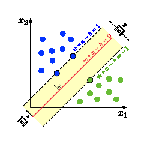
\includegraphics[width=.6\textwidth, height=.6\textheight, keepaspectratio]{svm_margin}
	\caption[SVM Hyperplane margin]{SVM Hyperplane with the associated margin formula}
	\label{fig:svm_margin}
\end{figure}

\subsection{SVM for authorship attribution}
Unlike currently used
classification approaches, like neural networks or decision trees, it allows for the processing of hundreds of thousands of features. This offers the opportunity to use all words of a text as inputs instead of a few hundred carefully selected characteristic words only. In similar text classification problems aiming at thematic categorization, the SVM has been shown to be quite effective \cite{joachims1998making}, \cite{dumais1998inductive}.
A SVM is able to classify a text with respect to content. In the framework of author attribution, it is not clear whether a specific topic addressed by the author or the structural or stylistic features of the authors language lead to a successful classification.
Among the earliest methods to be applied were various types of neural networks, typically using small sets of FWs as features \cite{holmes1995forensic}.
More recently, \cite{hirst2007bigrams} used neural networks on a wide variety of features. Other studies have used k-nearest neighbor \cite{zhao2005effective}, support vector machines \cite{diederich2003authorship}, \cite{koppel2005determining}, \cite{zheng2006framework}, and Bayesian regression \cite{madigan2005author}.
Comparative studies on machine learning methods for topic-based text categorization problems \cite{dumais1998inductive}, \cite{joachims1998making} have shown that in general, support vector machine (SVM) learning is at least as good for text categorization as any other
learning method, and the same has been found for authorship attribution \cite{zheng2006framework}.
The distinctive advantage of the SVM for text categorization is its ability to process many thousand different inputs. This opens the opportunity to use all words
in a text directly as features. For each word $w_i$ the number of times of occurrence is recorded. Typically a corpus contains more than 100,000 different words,
with each text covering only a small fraction.
\citeauthor{joachims1998making} \cite{joachims1998making} used the SVM for the classification of text into different topic categories. As features he uses word stems. To establish statistically significant features he requires that each feature occurs at least three times in a text. The empirical evaluation was done
on two test collections: the Reuter-21578 news agency
data set covering different topics and the Ohsumed corpus of William Hersh describing diseases. Using about 10000 features in every case, the two SVM versions (polynomial and rbf) performed substantially better than the currently best performing conventional methods (naive Bayes, Rocchio, decision trees, k-nearest
neighbor). \citeauthor{joachims1999transductive} \cite{joachims1999transductive} used a transductive SVM for text categorization which is able to exploit the information in unlabeled training data.
\citeauthor{dumais1998inductive} \cite{dumais1998inductive} use linear SVMs for text categorization because they are both accurate and fast. They are 35 times faster to train than the next most accurate (a decision tree) of the tested classifiers. They applied SVMs to the Reuter-21578 collection, emails and web pages.
\citeauthor{drucker1999support} \cite{drucker1999support} classify emails as spam and non spam. They find that boosting trees and SVMs have similar performance in terms of accuracy and speed. SVMs train significantly faster.

\section{RCV1 studies}
\cite{cheng2011author}
Reuters newsgroup dataset
Reuters is the world’s largest international multimedia news
agency, providing myriad news and mutual fund information
available on Reuters.com, video, mobile, and interactive television platforms. Reuters Corpus Volume 1 (RCV1) is drawn
from one of those online databases (Online, 2000). This dataset
consists of all English language stories produced by Reuters
journalists between August 20, 1996 and August 19, 1997. The
dataset is made available on two CD-ROMs and has been
formatted in XML by Reuters, Ltd. in 2000, for research
purposes. Both the archiving process and later preparation of
the XML dataset involved substantial verification and validation of the content, attempts to remove spurious or duplicated
documents, normalization of dateline and byline formats,
addition of copyright statements, and so on. The stories cover
a range of content typical of a large English language international newswire. They vary from a few hundred to several
thousand words in length.
We retrieved the information of the authors, categorized
the documents by the gender of the journalists, and discarded
the documents written by authors whose gender could not be
ascertained (e.g., neutral names). The text messages were
then extracted by removing unnecessary information (such as
date and time) and all XML formatting. Then we kept only the
messages that contained more than 200 but less than 1000
words. Since most messages in the Reuters Corpus were
newswire stories, these messages contained several quotes
from others, which could bias the accuracy of the gender
classifier. Therefore, we removed those messages that had too
many quotations (”) by setting the threshold of number of
quotes/character counts to be 0.002. Table 1 summarizes the
corpus used in our analysis.

Other corpus used to test our proposal was The Reuters
Corpus Volume 1 (RCV1) (Lewis et al. 2004). It consists of
a collection of newswire stories written in English that cover
four main topics: corporate/industrial (CCAT), economics
(ECAT), government/social (GCAT) and markets (MCAT).
Although it was not compiled for authorship attribution task,
it has been adapted to this task in previous works. For example, in Stamatatos (2008); Plakias and Stamatatos (2008) the
10 most prolific authors were chosen from the CCAT category, and then, 50 examples per author for training and 50
examples for testing were selected randomly with no overlapping between training and testing sets. In further sections,
we will reference to this corpus as RCV1-10.
In Houvardas and Stamatatos(2006), the authors proposed
another adaptation of the RCV1 corpus for the authorship
attribution task. They choose the 50 most prolific authors
from the Reuters Corpus, keeping 50 examples per author
for training and 50 examples per author for testing with no
overlapping between them. We will refer to this corpus as
RCV1-50.
The RCV1-10 and RCV1-50 datasets are both balanced
over different authors and have their genre fixed to news.
The main category of the news in both cases is fixed to corporate/industrial, but there are many subtopics covered in
the news and the length of the texts is short (from 2 to 8
KBytes). These corpora resemble a more realistic scenario,
when the amount of texts is limited and the number of candidate authors is large.
In 2000, a large corpus for the English language, the Reuters Corpus Volume 1
(RCV1) including over 800,000 newswire stories, become available for research
purposes. A natural application of this corpus is to be used as test bed for topic-based
text categorization tasks [18] since each document has been manually classified into a
series of topic codes (together with industry codes and region codes). There are four
main topic classes: CCAT (corporate/industrial), ECAT (economics), GCAT
(government/social), and MCAT (markets). Each of these main topics has many
subtopics and a document may belong to a subset of these subtopics. Although, not
particularly designed for evaluating author identification approaches, the RCV1
corpus contains ‘by-lines’ in many documents indicating authorship. In particular,
there are 109,433 texts with indicated authorship and 2,361 different authors in total.
RCV1 texts are short (approximately 2KBytes – 8KBytes), so they resemble a realworld author identification task where only short text samples per author may be
available. Moreover, all the texts belong to the same text genre (newswire stories), so
the genre factor is reduced in distinguishing among the texts. On the other hand, there
are many duplicates (exactly the same or plagiarized texts). The application of Rmeasure to the RCV1 text samples has revealed a list of 27,754 duplicates [19].
The RCV1 corpus has already been used in author identification experiments. In
[19] the top 50 authors (with respect to total size of articles) were selected. Moreover,
in the framework of the AuthorID project, the top 114 authors of RCV1 with at least
200 available text samples were selected [20]. In contrast to these approaches, in this
study, the criterion for selecting the authors was the topic of the available text
samples. Hence, after removing all duplicate texts found using the R-measure, the top 50 authors of texts labeled with at least one subtopic of the class CCAT
(corporate/industrial) were selected. That way, it is attempted to minimize the topic
factor in distinguishing among the texts. Therefore, since steps to reduce the impact of
genre have been taken, it is to be hoped that authorship differences will be a more
significant factor in differentiating the texts. Consequently, it is more difficult to
distinguish among authors when all the text samples deal with similar topics rather
than when some authors deal mainly with economics, others with foreign affairs etc.
The training corpus consists of 2,500 texts (50 per author) and the test corpus includes
other 2,500 texts (50 per author) non-overlapping with the training texts. \cite{houvardas2006n}

\subsection{Studies on RCV1 on authorship attribution}

\section{GDELT studies}
The GDELT Project is one of the largest publicly available digitized book database
which has more than 3.5 million books published from 1800-2015. The GDELT
Project is an open platform for research and analysis of global society and thus all
datasets released by the GDELT Project are available for unlimited and unrestricted
use for any academic, commercial, or governmental use of any kind without any
fee\footnote{\url{https://www.gdeltproject.org/about.html}}. The whole digitized dataset is publicly available and interested researchers
can freely perform SQL queries using the Google big query platform. For example;
the book names, publication year, quotations, themes, the original text of the book
of “Mark Twain” which were written between 1890 to 1900 can be found as follows
using the Big query platform of Google.
To decrease the bias and create a reliable dataset the following criteria have been
chosen to filter out authors: English language writing authors, authors that have
enough books available (at least 5), 19th century authors. With these criteria 50
authors have been selected and their books were queried through Big Query Gdelt
database. The next task has been cleaning the dataset due to OCR reading problems
in the original raw form. To achieve that, firstly all books have been scanned through
to get the overall number of unique words and each words frequencies. While scanning
the texts, the first 500 words and the last 500 words have been removed to take out
specific features such as the name of the author, the name of the book and other word
specific features that could make the classification task easier. After this step, we have
chosen top 10, 000 words that occurred in the whole 50 authors text data corpus. The
words that are not in top 10, 000 words were removed while keeping the rest of the
sentence structure intact.
Afterwards, the words are represented with numbers from
1 to 10, 000 reverse ordered according to their frequencies. The entire book is split
into text fragments with 1000 words each. We separately maintained author and
book identification number for each one of them in different arrays. Text segments
with less than 1000 words were filled with zeros to keep them in the dataset as well.
1000 words make approximately 2 pages of writing, which is long enough to extract a variety of features from the document. The reason why we have represented top
10, 000 words with numbers is to keep the anonymity of texts and allow researchers
to run feature extraction techniques faster. Dealing with large amounts of text data
can be more challenging than numerical data for some feature extraction techniques.
In order to make the AA problem more realistic, when splitting the training and
testing dataset the writings of George Eliot (5), Jack London (7), Frances Hodgson
Burnett (31), Sarah Stickney Ellis (47), Thomas Nelson Page (49) have been removed
from the training and added to testing set. This creates a non-exhaustive training set
with 45 authors while the test set contains 50 authors. In total this leads to 53678
training data instances, 39922 testing data instances. Each of these instances consist
of 1000 words text fragment. Another important aspect we have considered while
splitting training and testing data is to keep all fragments of the same book either in
the training or testing dataset. This way we do not end up training and testing on the
same books. Without this restriction the classification task would be much simpler
and simple bag of words representation with SVM would give much higher F-1 scores.
To study the sentence structure and writing style from a different perspective, the
same steps also have been applied to create another dataset in which stop words have
been removed while keeping the word order same for the remaining words.
\subsection{Authorship attribution GDELT}

\section{The guardian studies}

\subsection{Cross-topic authorship attribution}

\section{Studies on Stanford Amazon Food Reviews}

\section{Dataset selection}